% Fig. 2: decision path that names the drift type, one journal column (83.5 mm) wide.
\documentclass[border=0.5pt]{standalone}
\usepackage{newtxtext}
\usepackage{tikz}
\usetikzlibrary{arrows.meta}
\begin{document}
\fontsize{8}{9.2}\selectfont
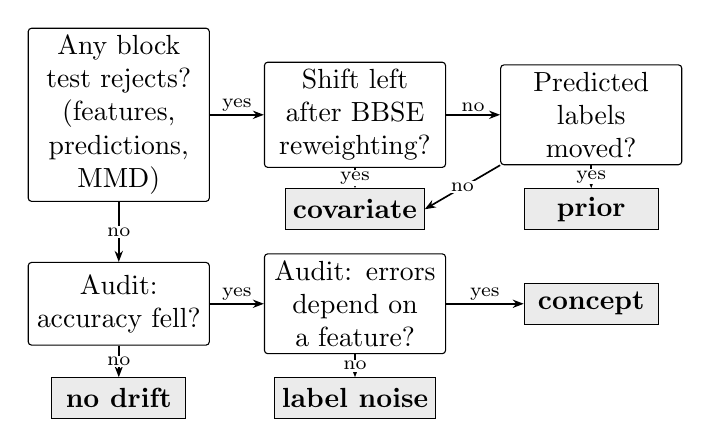
\begin{tikzpicture}[
  q/.style={draw, rounded corners=1.2pt, align=center, inner sep=0.9mm, text width=21.2mm, minimum height=10.5mm,
            execute at begin node={\hyphenpenalty=10000}},
  v/.style={draw, fill=black!8, align=center, inner sep=0.9mm, minimum width=17mm, minimum height=5.2mm, font=\bfseries},
  flow/.style={-{Stealth[length=1.4mm]}, semithick},
  lab/.style={font=\fontsize{7}{8}\selectfont, midway, fill=white, inner sep=0.6pt},
  hlab/.style={font=\fontsize{7}{8}\selectfont, midway, above, inner sep=0.8pt}]
\node[q] (q1) at (0,0)        {Any block test rejects? (features, predictions, MMD)};
\node[q] (q2) at (30mm,0)     {Shift left after BBSE reweighting?};
\node[q] (q3) at (60mm,0)     {Predicted labels moved?};
\node[v] (cov) at (30mm,-12mm) {covariate};
\node[v] (pri) at (60mm,-12mm) {prior};
\node[q] (q4) at (0,-24mm)    {Audit: accuracy fell?};
\node[q] (q5) at (30mm,-24mm) {Audit: errors depend on a feature?};
\node[v] (con) at (60mm,-24mm) {concept};
\node[v] (non) at (0,-36mm)    {no drift};
\node[v] (noi) at (30mm,-36mm) {label noise};
\draw[flow] (q1) -- node[hlab]{yes} (q2);
\draw[flow] (q2) -- node[lab]{yes} (cov);
\draw[flow] (q2) -- node[hlab]{no} (q3);
\draw[flow] (q3) -- node[lab]{yes} (pri);
\draw[flow] (q3.south west) -- node[lab]{no} (cov.east);
\draw[flow] (q1) -- node[lab]{no} (q4);
\draw[flow] (q4) -- node[hlab]{yes} (q5);
\draw[flow] (q4) -- node[lab]{no} (non);
\draw[flow] (q5) -- node[hlab]{yes} (con);
\draw[flow] (q5) -- node[lab]{no} (noi);
\end{tikzpicture}
\end{document}
